\documentclass[a4paper]{article}
\usepackage[affil-it]{authblk}
\usepackage[backend=bibtex,style=numeric]{biblatex}
\usepackage{geometry}
\usepackage{amsmath}
\usepackage{float, caption}
\usepackage{graphicx}
\geometry{margin=1.5cm, vmargin={0pt,1cm}}
\setlength{\topmargin}{-1cm}
\setlength{\paperheight}{29.7cm}
\setlength{\textheight}{25.3cm}

\addbibresource{citation.bib}

\begin{document}
% =================================================
\title{Numerical Analysis homework \# 3}

\author{Guang Zhang 3230105121
  \thanks{Electronic address: \texttt{zhuiguang49@foxmail.com}}}
\affil{(Information and Computing Science, Class XJ2301), Zhejiang University }

\date{Due time: \today}

\maketitle






% ============================================
\section*{I. Question I}


Let $p(x)=a_0+a_1x+a_2x^2+a_3x^3$, then its first derivative would be $p'(x)=a_1+2a_2x+3a_3x^2$, its second derivative would be $p''(x)=2a_2+6a_3x$. And we denote $q(x)=(2-x)^3$, its first derivative would be
$q'(x)=-3(2-x)^2$, its second derivative would be $q''(x)=6(2-x)$. Due to the $C^2$ continuity condition, we can obtain that $p(1)=q(1)$, that is to say

\begin{align}
  a_0+a_1+a_2+a_3=1 \label{eq:C2连续性条件1}\\
  a_1+2a_2+3a_3=-3  \label{eq:C2连续性条件2}\\
  2a_2+6a_3=6       \label{eq:C2连续性条件3}
\end{align}
And it easy to grasp that $p(0)=a_0=q(0)=0$. By equation(\ref{eq:C2连续性条件1})(\ref{eq:C2连续性条件2})(\ref{eq:C2连续性条件3}), we can obtain that $a_1=12,a_2=-18,a_3=7$, which implies that $p(x)$ satisfies
\begin{equation}
  p(x) = 12x-18x^2+7x^3 \label{eq:p(x)}
\end{equation}
By the definition of natural cubic spline, we have $s''(0)=s''(2)$. However, by comupting we can obtain that $s''(2)=0$, while $s''(0)=-36\neq 0$, which is contrary to the definition of natural cubic spline, so $s(x)$ is not a natural cubic spline.  


\section*{II. Question II}

\subsection*{II.a}

In the $n-1$ interval $[x_i,x_{i+1}]$, the spline $s(x)$ is a quadratic polynomial, we denote it as $p_i(x)=a_ix^2+b_ix+c_i$.
Since there are $n-1$ intervals and 3 unknown coefficients for each interval, thus we have a total of $3(n-1)$ unknown parameters.
While the definition of $s\in S_2^1$ provides the following constraints:

\begin{enumerate}
  \item The spline must pass through all the data points, that is, $s(x_i)=f_i$ holds for $i=1,2,\cdots,n$
  \item The polynomial pieces must join continuously at the $n-2$ internal knots, which can give us $n-2$ conditions, that is $p_i(x_{i+1})=p_{i+1}(x_{i+1})$ holds for $i=1,2,\cdots,n-2$
  \item The first derivative must also be continuous at the $n-2$ internal knots, which can give us another $n-2$ conditions, that is, $p_i'(x_{i+1})=p_{i+1}'(x_{i+1})$ for $i=1,2,\cdots,n-2$ 
\end{enumerate}

To conclude, we have $3n-4$ constraints, while we have $3n-3$ unknown parameters, so the constraints is not enough to solve the unknown parametes. Therefore, an additional condition is needed to determine $s$ uniquely.

\subsection*{II.b}
In other words, we need to find the specific quadratic polynomial $p_i(x)$ on the interval $[x_i,x_{i+1}]$ given three pieces of Information:
\begin{enumerate}
  \item $p_i(x_i) = s(x_i)=f_i$
  \item $p_i(x_{i+1}) = s(x_{i+1})=f_{i+1}$
  \item $p_i'(x_i)=s'(x_i)=m_i$
\end{enumerate}
We can use Newton form to to construct this polynomial centered at $x_i$, that is to say
\begin{equation}
  p_i(x)=C_0+C_1(x-x_i)+C_2(x-x_i)^2
\end{equation}
Then the derivative of $p_i(x)$ is $p_i'(x)=C_1+2C_2(x-x_i)$. Since $p_i(x_i)=f_i,p_i'(x_i)=m_i$, we can obtain that $C_0=f_i,C_1=m_i$, then $p_i(x)$ can be written as
\begin{equation}
  p_i(x)=f_i+m_i(x-x_i)+C_2(x-x_i)^2
\end{equation}
In addition, we have $p_{i}(x_{i+1})=f_i+m_i(x_{i+1}-x_i)+C_2(x_{i+1}-x_i)^2=f_{i+1}$, we can obtain that $C_2$ satisfies
\begin{equation}
  C_2=\frac{f_{i+1}-f_i-m_i(x_{i+1}-x_i)}{(x_{i+1}-x_i)^2}
\end{equation}
Finally, we have
\begin{equation}
  p_i(x)=f_i+m_i(x-x_i)+\frac{f_{i+1}-f_i-m_i(x_{i+1}-x_i)}{(x_{i+1}-x_i)^2}(x-x_i)^2 \label{eq:conclusion}  
\end{equation}


\subsection*{II.c}

By definition, we have $m_{i+1}=s'(x_{i+1})=p_{i+1}'(x_{i+1})$, due to the $C^1$ continuity, we have $m_{i+1}=p_i'(x_{i+1})$, and we can use the conclusion of II.b, that is equation(\ref{eq:conclusion}), we have
\begin{equation}
  m_{i+1}=p_{i}'(x_{i+1})=m_i+2\frac{f_{i+1}-f_i}{x_{i+1}-x_i}-2m_i
\end{equation}
The equation can be turned into a recursive formula
\begin{equation}
  m_{i+1}=2\frac{f_{i+1}-f_i}{x_{i+1}-x_i}-m_i \label{eq:recursive}
\end{equation}
Since $m_1=f'(a)$ is given, we can compute $m_2,m_3,m_{n-1}$ recursively by equation(\ref{eq:recursive})

\section*{III. Question III}

Let $s_2(x)$ be $s_2(x)=a_0+a_1x+a_2x^2+a_3x^3$, then its first derivative and second derivative would be $s_2'(x)=a_1+2a_2x+3a_3x^2,s''_2(x)=2a_2+6a_3x$, and the first, second derivative of $s_1(x)$ is $s'_1(x)=3c(x+1)^2,s_1''(x)=6c(x+1)$.
Since $s(x)$ is a natural cubic spline on $[-1,1]$, and a natural spline must have $C^2$ continuity at all internal knots and must have zero second derivatives at the endpoints, while $s''(-1)=0$ is automatically satisfied. So we try to satisfy the $C^0,C^1,C^2$ continuity, we can obtain that
\begin{itemize}
  \item $s_1(0)=1+c=s_2(0)=a_0$
  \item $s_1'(0)=3c=s_2'(0)=a_1$
  \item $s_1''(0)=6c=s_2''(0)=2a_2$ 
  \item $s''(1)=s_2''(1)=2a_2+6a_3=0$
\end{itemize}
Thus, we have $a_0=c-1,a_1=3c,a_2=3c,a_3=-c$, then $s_2(x)$ can be written as $s_2(x)=1+c+3cx+3cx^2-cx^3$
Furthermore, we have $s(1)=1+c+3c+3c-c=-1$, from which we can obtain that $c=-\frac{1}{3}$
\section*{IV. Question IV}
\subsection*{IV.a}
We have $f_0=f(-1)=\cos(-\frac{\pi}{2})=0$, $f_1=f(0)=\cos(0)=1$, $f_2=f(1)=\cos(\frac{\pi}{2})=0$. And we denote $s(x)$ is defined by $s_0(x)$ on $[-1,0]$, $s_1(x)$ on $[0,1]$, while $M_i=s''(x_i)$ is the second derivatives at the knots. Then the natural boundary conditions would be $M_0=s''(-1)=0,M_2=s''(1)=0$, and the knot spacing would be $h_0=x_1-x_0=1,h_1=x_2-x_1=1$ 
We can use the standard system of euqations for cubic splines. For the single internal knot $x_1=0$, we can obtain that
\begin{equation}
  h_0M_0+2(h_0+h_1)M_1+h_1M_2=6(\frac{f_2-f_1}{h_1}-\frac{h_1-f_0}{h_0})
\end{equation}
By substituting $h_0,h_1,M_0,M_2$, we can obtain that $M_1=-3$, thus, the second derivatives at the knots are $(M_0,M_1,M_2)=(0,-3,0)$. Then, we can use the general formula for a spline segments $s_i(x)$
on the interval $[x_i,x_{i+1}]$, that is to say
\begin{equation}
  s_i(x)=M_i\frac{(x_{i+1}-x)^3}{6h_i} + M_{i+1}\frac{(x-x_i)^3}{6h_i}+(\frac{f_i}{h_i}-\frac{M_ih_i}{6})(x_{i+1}-x_i)+(\frac{f_{i+1}}{h_i}-\frac{M_{i+1}h_i}{6})(x-x_i) \label{eq:waiting substituting}
\end{equation}
Then for $s_0(x)$ on $[-1,0]$, we have $x_i=-1,x_{i+1}=0, h_i=1,f_i=0,f_{i+1}=1, M_i=0,M_{i+1}=-3$, by substituting into equation(\ref{eq:waiting substituting}), we can obtain that
\begin{eqnarray}
  s_0(x)=-\frac{1}{2}x^3-\frac{3}{2}x^2+1
\end{eqnarray}
For $s_1(x)$ on $[0,1]$, we have $x_i=0,x_{i+1}=1,h_i=1,f_i=1,f_{i+1}=0,M_i=-3,M_{i+1}=0$, by substituting into euqation(\ref{eq:waiting substituting}), we can obtain that 
\begin{equation}
  s_1(x)=\frac{1}{2}x^3-\frac{3}{2}x^2+1
\end{equation}
Thus, we can get a natural cubic spline interpolant 

\begin{equation}
  s(x)=\begin{cases}
    -\frac{1}{2}x^3-\frac{3}{2}x^2+1,&x\in[-1,0]\\
    \frac{1}{2}x^3-\frac{3}{2}x^2+1,&x\in[0,1]
  \end{cases}
\end{equation}


\subsection*{IV.b}

$g(x)$ is the quadratic polynomial that interpolates $f$ at $(-1,0),(0,1),(1,0)$, we denote $g(x)$ as $g(x)=a+bx+cx^2$. Then we have
\begin{align}
  g(0)=a=1\\
  g(1)=a+b+c=0\\
  g(-1)=a-b+c=0
\end{align}
Then we can obtain that $c=-1,b=0,a=1$, that is, $g(x)=1-x^2$.\newline
To caculate $E(s)$, we need to find the second derivatives of $s(x)$, we have $s'_0(x)=-\frac{3}{2}x^2-3x,s_0''(x)=-3x-3,s'_1(x)=\frac{3}{2}x^2-3x,s_1''(x)=3x-3$, then we can integrate $[s''(x)]^2$ over the full interval:
\begin{equation}
  E(s)=\int_{-1}^0[s_0''(x)]^2dx+\int_{0}^{1}[s_1''(x)]^2dx=6
\end{equation}
\newline To caculate $E(g)$, we have 
\begin{equation}
  E(g)=\int_{-1}^{1}[g''(x)]^2 dx = \int_{-1}^1(-2)^2dx = 8
\end{equation}
\newline To caculate $E(f)$, we have
\begin{equation}
  E(f) = \int_{-1}^{1}[f''(x)]^2dx=\int_{-1}^1(-\frac{\pi^2}{4}\cos(\frac{\pi}{2}x))^2dx=\frac{\pi^4}{16}  
\end{equation}
While $E(f)=\frac{\pi^4}{16}\approx 6.088$, it is easy to obatin that $E(s)<E(f),E(s)<E(g)$, the minimal energy property is verified.

\section*{V. Question V}

\subsection*{V.a}
We can use the Cox-de Boor formula. The $B_i^2(x)$ spline is bulit from $B_i^1(x)$ and $B_{i+1}^1(x)$. The recurrence relation is 
\begin{equation}
  B_i^2(x)=\frac{x-t_{i-1}}{t_{i+1}-t_{i-1}}B_i^1(x)+\frac{t_{i+2}-x}{t_{i+2}-t_i}B_{i+1}^1(x)
\end{equation}
And the basic functions $B_i^1(x)$ and $B_{i+1}^1(x)$ are defined as follows:

\begin{align}
  B_i^1(x)=\begin{cases}
    \frac{x-t_{i-1}}{t_i-t_{i-1}},& x\in[t_{i-1},t_i]\\
    \frac{t_{i+1}-x}{t_{i+1}-t_i}, & x\in[t_i,t_{i+1}]\\
    0 & otherwise
  \end{cases}\\
  B_{i+1}^1(x)=\begin{cases}
    \frac{x-t_i}{t_{i+1}-t_i},&x\in[t_i,t_{i+1}]\\
    \frac{t_{i+2}-x}{t_{i+2}-t_{i+1}},& x\in[t_{i+1},t_{i+2}]\\
    0 &otherwise
  \end{cases}
\end{align}
Thus, we can derive $B_i^2(x)$ by combining these over its full support $[t_{i-1},t_{i+2}]$.\newline
For $x\in[t_{i-1},t_i]$, we have 
\begin{equation}
  B_{i+1}^1(x)=0,   
\end{equation}
and
\begin{equation}
  B_{i}^2(x)=\frac{x-t_{i-1}}{t_{i+1}-t_{i-1}}(\frac{x-t_{i-1}}{t_i-t_{i-1}}) \label{eq:26}
\end{equation}
For $x\in[t_i,t_{i+1}]$, we have
\begin{equation}
  B_i^2(x)=\frac{x-t_{i-1}}{t_{i+1}-t_{i-1}}(\frac{t_{i+1}-x}{t_{i+1}-t_{i}})+\frac{t_{i+2}-x}{t_{i+2}-t_i}(\frac{x-t_i}{t_{i+1}-t_i}) \label{eq:27}
\end{equation}
For $x\in [t_{i+1},t_{i+2}]$, we have
\begin{equation}
  B_i^2(x)=0+\frac{t_{i+2}-x}{t_{i+2}-t_i}(\frac{t_{i+2}-x}{t_{i+2}-t_{i+1}}) \label{eq:28}
\end{equation}
Otherwise, $B_i^2(x)=0$
\subsection*{V.b}
First, we can compute the derivative $\frac{d}{dx}B_i^2(x)$ for each piece, for simplicity, we denote $w_i=t_{i+1}-t_i$.\newline
For $x\in(t_{i-1},t_i)$, $\frac{d}{dx}B_i^2(x)=\frac{2(x-t_{i-1})}{w_i(t_i-t_{i-1})}$;\newline
For $x\in(t_{i},t_{i+1})$, $\frac{d}{dx}B_i^2(x)=\frac{d}{dx}[\frac{(x-t_{i-1})(t_{i+1}-x)}{w_i(t_{i+1}-t_i)}]=\frac{t_{i+1}+t_{i-1}-2x}{w_i(t_{i+1}-t_i)}+\frac{t_{i+2}+t_i-2x}{w_{i+1}(t_{i+1}-t_{i})}$;\newline
For $x\in(t_{i+1},t_{i+2})$, $\frac{d}{dx}B_i^2(x)=\frac{-2(t_{i+2}-x)}{w_{i+1}(t_{i+2}-t_{i+1})}$;\newline
Then it is easy to obtain that at knot $t_i$, we have:
\begin{align}
  \lim_{x\to t_i^{-}}\frac{d}{dx}B_i^2(x)&=\frac{2(t_i-t_{i-1})}{w_i(t_i-t_{i-1})}=\frac{2}{t_{i+1}-t_{i-1}}\\
  \lim_{x\to t_i^+}\frac{d}{dx}B_i^2(x)&=\frac{t_{i+1}+t_{i-1}-2t_i}{w_i(t_{i+1}-t_i)}+\frac{t_{i+2}+t_i-2t_i}{w_{i+1}(t_{i+1}-t_i)}=\frac{2}{t_{i+1}-t_{i-1}}\\
\end{align}
So the derivative is continuous at $t_i$.\newline
At knot $t_{i+1}$, we have:
\begin{align}
  \lim_{x\to t_{i+1}^-}\frac{d}{dx}B_i^2(x)&=\frac{-t_{i+1}+t_{i-1}}{(t_{i+1}-t_{i-1})(t_{i+1}-t_i)}+\frac{t_{i+2}+t_{i}-2t_{i+1}}{w_{i+1}(t_{i+1}-t_i)}=\frac{-2}{t_{i+2}-t_{i}}\\
  \lim_{x\to t_{i+1}^{+}}\frac{d}{dx}B_i^2(x)&=\frac{-2(t_{i+2}-t_{i+1})}{w_{i+1}(t_{i+2}-t_{i+1})}=\frac{-2}{t_{i+2}-t_{i}}
\end{align}
So the derivative is continuous at $t_{i+1}$.

\subsection*{V.c}
From V.b, we have $\frac{d}{dx}B_i^2(x)=\frac{2(x-t_{i-1})}{w_i(t_i-t_{i-1})}$ when $x\in(t_{i-1},t_i)$, so $\frac{d}{dx}B_i^2(x)>0$ holds for all $x\in(t_{i-1},t_i)$, which means the function is increasing.\newline
And we have $\frac{d}{dx}B_i^2(x)=\frac{-2(t_{i+2}-x)}{w_{i+1}(t_{i+2}-t_{i+1})}$ when $x\in(t_{i+1},t_{i+2})$, so $\frac{d}{dx}B_i^2(x)<0$ holds for all $x\in(t_{i+1},t_{i+2})$, which means the function is decreasing.\newline
Since the function is increasing in $(t_{i-1},t_i)$ and decresing at $(t_{i+1},t_{i+2})$, then the single critical point $x^{*}$ must lie in the middle interval $(t_{i},t_{i+1})$. Let the derivative on $x^{*}$ be zero, we can obtain that 
\begin{equation}
  \frac{t_{i+1}+t_{i-1}-2x^{*}}{t_{i+1}-t_{i-1}}+\frac{t_{i+2}+t_i-2x^{*}}{t_{i+2}-t_i}=0
\end{equation}
from which we can solve $x^{*}$, and $x^{*}$ satisfies
\begin{equation}
  x^{*}=\frac{t_{i+1}t_{i+2}-t_it_{i-1}}{t_{i+2}+t_{i+1}-t_i-t_{i-1}}
\end{equation}
\subsection*{V.d}
First of all, we prove that $B_i^2(x)\geq 0$. By equation(\ref{eq:26})(\ref{eq:27})(\ref{eq:28}), it is easy to obtain that $B_i^2(x)\geq 0$, because each factor is non-negative.\newline
Then we prove that $B_i^2(x)\leq 1$, we can use the B-splines $B_i^k(x)$'s partition of unity, that is $\sum_iB_i^k(x)=1$ for all $x$ in the domain. Since $\sum_i B_i^2(x)=1$, and $B_i^2(x)\geq 0$ holds, then it is easy to obtain $B_i^2(x)\leq 1$ holds.\newline
Therefore, $B_i^2(x)\in[0,1]$

\subsection*{V.e}

\begin{figure}[H]
  \centering
  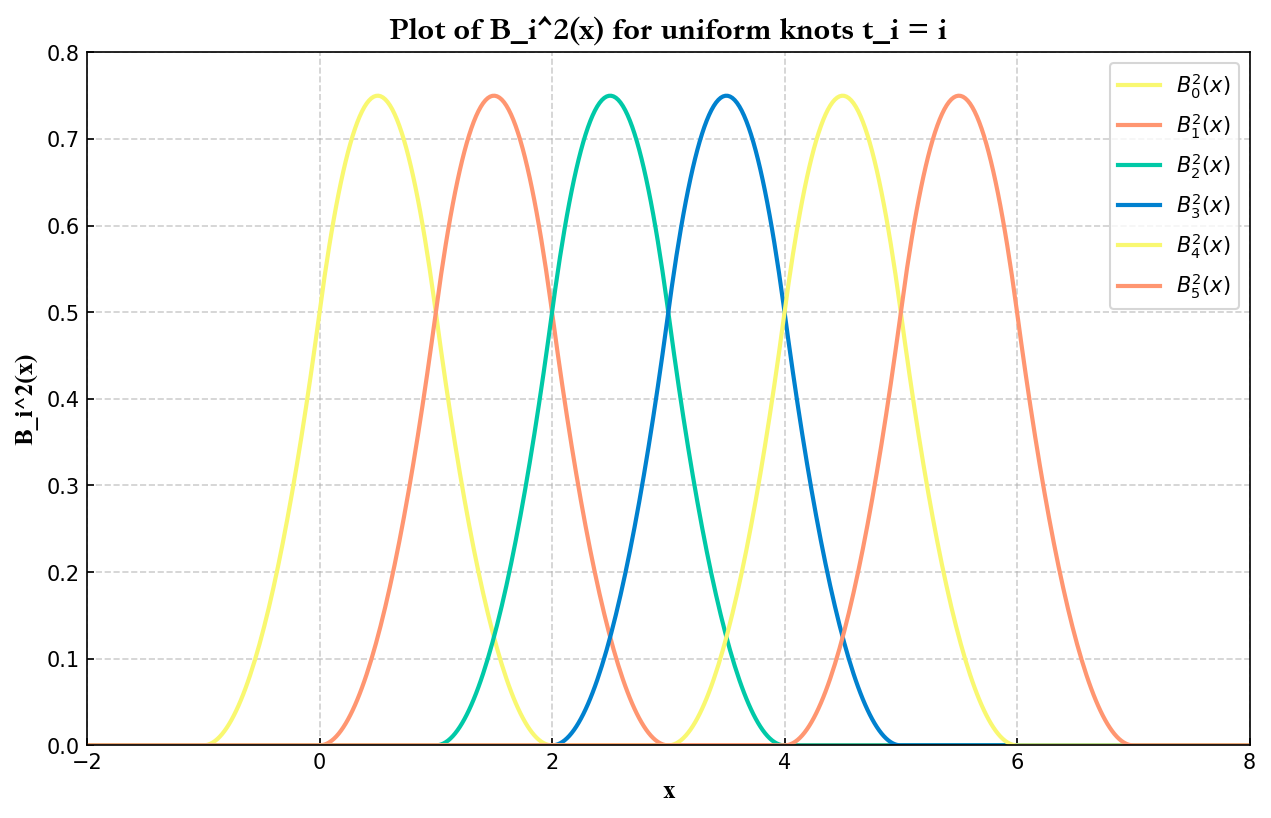
\includegraphics[width=0.8\textwidth]{quadratic_b_spline_plot.png} 
  \caption{Plot of $B_i^2(x)$ for uniform knots $t_i = i$.}
\end{figure}

This plot illustrates a series of quadratic B-spline basis functions, $B_i^2(x)$, under the condition uniform knots $t_i=i$

\section*{VI. Question VI}

Let $f(t)=(t-x)^2_{+}$, LHS can be expanded using the definition of divided differences:
\begin{equation}
  LHS=(t_{i+2}-t_{i-1})\frac{[t_i,t_{i+1},t_{i+2}]f-[t_{i-1},t_i,t_{i+1}]f}{t_{i+2}-t_{i-1}}=[t_i,t_{i+1},t_{i+2}]f-[t_{i-1},t_i,t_{i+1}]f
\end{equation}
And RHS is the definition of $B_i^2(x)$ as we derived in V.a4paper
The problem can be divided into several cases as below:
\begin{itemize}
  \item Case1: $x\geq t_{i+2}$, then for all $t\in\{t_{i-1},t_i,t_{i+1},t_{i+2}\}$, we have $t\leq t_{i+2}\leq x$, which means $f(t)=(t-x)^2_{+}=0$ holds for all knots. Then we have LHS$=$RHS$=0$
  \item Case2: $x<t_{i-1}$, then for all $t\in\{t_{i-1},t_i,t_{i+1},t_{i+2}\}$, we have $t\geq t_{i-1}>x$, which means $f(t)=(t-x)^2_+=(t-x)^2$, while the 3-order divided differences of any quadratic is zero, that is,
  LHS $=$ 0, while $B_i^2(x)=0$ holds too, that is, RHS $=0$, so we have LHS $=$ RHS
  \item Case3: $x\in[t_{i+1},t_{i+2})$, then we have $f(t_{i-1})=0,f(t_i)=0,f(t_{i+1})=0,f(t_{i+2})=(t_{i+2}-x)^2$, then we consider LHS $[t_i,t_{i+1},t_{i+2}]f-[t_{i-1},t_i,t_{i+1}]f$, we can obtain that
    \begin{align}
      [t_{i-1},t_i,t_{i+1}]f=\frac{[t_i,t_{i+1}]f-[t_{i-1},t_i]f}{t_{i+1}-t_{i-1}}=0\\
      [t_i,t_{i+1},t_{i+2}]f=\frac{[t_{i+1},t_{i+2}]f-[t_i,t_{i+1}]f}{t_{i+2}-t_i}=\frac{\frac{f(t_{i+2}-f(t_{i+1}))}{t_{i+2}-t_{i+1}}-0}{t_{i+2}-t_i}=\frac{(t_{i+2}-x)^2}{(t_{i+2}-t_i)(t_{i+2}-t_{i+1})}
    \end{align}
  Which means LHS $=\frac{(t_{i+2}-x)^2}{(t_{i+2}-t_i)(t_{i+2}-t_{i+1})}=$ RHS
  \item Case4: $x\in[t_{i-1},t_i)$, then we have $f(t_{i-1})=0, f(t_i)=(t_i-x)^2,f(t_{i+1})=(t_{i+1}-x)^2,f(t_{i+2})=(t_{i+2}-x)^2$, then we consider LHS $[t_i,t_{i+1},t_{i+2}]f-[t_{i-1},t_i,t_{i+1}]f$, we can obtain that
    \begin{align}
      [t_i,t_{i+1},t_{i+2}]f=1\\
      [t_{i-1},t_{i},t_{i+1}]f = \frac{t_{i+1}+t_i-2x-\frac{(t_i-x)^2}{t_i-t_{i-1}}}{t_{i+1}-t_{i-1}}
    \end{align}
    Thus, by simplification, we can obtain that LHS $=\frac{(x-t_{i-1})^2}{(t_{i+1}-t_{i-1})(t_i-t_{i-1})}= $ RHS
  \item Case5: $x\in[t_i,t_{i+1})$, we have $f(t_{i-1})=0,f(t_i)=0,f(t_{i+1})=(t_{i+1}-x)^2,f(t_{i+2})=(t_{i+2}-x)^2$, then we consider LHS $[t_i,t_{i+1},t_{i+2}]f-[t_{i-1},t_i,t_{i+1}]f$, we can obtain that
  \begin{align}
    [t_{i-1},t_i,t_{i+1}]f=\frac{[t_i,t_{i+1}]f-[t_{i-1},t_i]f}{t_{i+1}-t_{i-1}}=\frac{(t_{i+1}-x)^2}{(t_{i+1}-t_{i-1})(t_{i+1}-t_i)}\\
    [t_i, t_{i+1}, t_{i+2}]f = \frac{[t_{i+1}, t_{i+2}]f - [t_i, t_{i+1}]f}{t_{i+2}-t_i} =\frac{\frac{(t_{i+2}-x)^2 - (t_{i+1}-x)^2}{t_{i+2}-t_{i+1}} - \frac{(t_{i+1}-x)^2}{t_{i+1}-t_i}}{t_{i+2}-t_i}
  \end{align}
  by simplification, we have LHS = $\frac{(x-t_{i-1})(t_{i+1}-x)}{(t_{i+1}-t_{i-1})(t_{i+1}-t_i)} + \frac{(t_{i+2}-x)(x-t_i)}{(t_{i+2}-t_i)(t_{i+1}-t_i)}=$ RHS 
\end{itemize} 

To conclude, the equation holds true for all possible intervals of $x$.


\section*{VII. Question VII}
According to Theorem 3.34 of the book, we have 
\begin{equation}
  \frac{d}{dx}B_i^{n+1}(x)=(n+1)(\frac{B_i^n(x)}{t_{i+n-t_{i-1}}}-\frac{B_{i+1}^n(x)}{t_{i+n+1}-t_i})
\end{equation}
Then we can obtain that 
\begin{equation}
  \int_{t_{i-1}}^{t_{i+n+1}}\frac{d}{dx}B_i^{n+1}(x)=(n+1)\int_{t_{i-1}}^{t_{i+n+1}}(\frac{B_i^n(x)}{t_{i+n-t_{i-1}}}-\frac{B_{i+1}^n(x)}{t_{i+n+1}-t_i})dx
\end{equation}
LHS$=[B_i^{n+1}(x)]_{t_{i-1}}^{t_{i+n+1}}=B_i^{n+1}(t_{i+n+1})-B_i^{n+1}(t_{i-1})=0$. Since LHS = 0, we have to prove RHS=0, which is equivalent to
\begin{equation}
  \int_{t_{i-1}}^{t_{i+n+1}}\frac{B_i^n(x)}{t_{i+n}-t_{i-1}}dx = \int_{t_{i-1}}^{t_{i+n+1}}\frac{B_{i+1}^n(x)}{t_{i+n+1}-t_i}dx
\end{equation}
And we need to be aware that the support of $B_i^n(x)$ is $[t_{i-1},t_{i+n}]$, and the support of $B_{i+1}^n(x)$ is $[t_i,t_{i+n+1}]$. so we just need to consider the intgegration in their own supports, that is:
\begin{equation}
  \int_{t_{i-1}}^{t_{i+n}}\frac{B_i^n(x)}{t_{i+n}-t_{i-1}}dx=\int_{t_i}^{t_{i+n+1}}\frac{B_{i+1}^n(x)}{t_{i+n+1}-t_i}dx
\end{equation}
which means that the scaled integral of $B_i^n(x)$ is identical to the scaled integral of $B_{i+1}^n(x)$. By recursion, we can prove that the value of the scaled integral is constant for all indices $i$.

\section*{VIII. Question VIII}

\subsection*{VIII.a}

By definition, we can obtain that $\tau_2(x_i,x_{i+1},x_{i+2})$ satisfies
\begin{equation}
  \tau_2(x_,x_{i+1},x_{i+2})=x_i^2+x_{i+1}^2+x_{i+2}^2+x_ix_{i+1}+x_ix_{i+2}+x_{i+1}x_{i+2}
\end{equation}
And then we can compute $[x_i,x_{i+1},x_{i+2}]x^4$, we have 
\begin{align}
  [x_i,x_{i+1}]x^4=\frac{x_{i+1}^4-x_i^4}{x_{i+1}-x_i}=x_{i+1}^3+x_{i+1}^2x_i+x_{i+1}x_i^2+x_i^3\\
  [x_{i+1},x_{i+2}]x^4=\frac{x_{i+2}^4-x_{i+1}^4}{x_{i+2}-x_{i+1}}=x_{i+2}^3+x_{i+2}^2x_{i+1}+x_{i+2}x_{i+1}^2+x_{i+1}^3
\end{align}
Then we can obtain that
\begin{equation}
  [x_i,x_{i+1},x_{i+2}]x^4=\frac{[x_{i+1},x_{i+2}]x^4-[x_i,x_{i+1}]x^4}{x_{i+2}-x_i}= x_{i+2}^2 + x_{i+2} x_i + x_i^2 + x_{i+1} x_{i+2} + x_{i+1} x_i + x_{i+1}^2
\end{equation}

Thus, we have verified LHS=RHS

\subsection*{VIII.b}

We can prove the theorem by induction. By Lemma 3.45 of the book, we have 
\begin{equation}
  \tau_k(x_i, \dots, x_{i+n}) = \frac{\tau_{k+1}(x_{i+1}, \dots, x_{i+n}) - \tau_{k+1}(x_i, \dots, x_{i+n-1})}{x_{i+n} - x_i}
\end{equation}
Let $P(n)$ be the proposition $[x_i,\cdots,x_{i+n}]x^m=\tau_{m-1}(x_i,\cdots,x_{i+n})$.\newline
When $n=0$, $[x_i]x^m = x_i^m=\tau_m(x_i)$, the base case holds.\newline
And we assmue $P(k)$ is true for $n=k$, where $k<m$, that is to say, for any $k$ knots, we have 
\begin{equation}
  [x_i,\cdots,x_{i+k}]x^m=\tau_{m-k}(x_i,\cdots,x_{i+k})
\end{equation}
Then we prove $P(k+1)$ is true, that is, $[x_i,\cdots,x_{i+k+1}]x^m=\tau_{m-k-1}(x_i,\cdots,x_{i+k+1})$
Through Lemma 3.45, we can obtain that
\begin{equation}
  \tau_{m-(k+1)}(x_i, \dots, x_{i+k+1}) = \frac{\tau_{m-k}(x_{i+1}, \dots, x_{i+k+1}) - \tau_{m-k}(x_i, \dots, x_{i+k})}{x_{i+k+1} - x_i}
\end{equation}
Then by applying the inductive hypothesis, we have $\tau_{m-k}(x_{i+1}, \dots, x_{i+k+1}) = [x_{i+1}, \dots, x_{i+k+1}]x^m$ and $\tau_{m-k}(x_i, \dots, x_{i+k}) = [x_i, \dots, x_{i+k}]x^m$
Then by substituting we have 
\begin{equation}
  \tau_{m-(k+1)}(x_i, \dots, x_{i+k+1}) = \frac{[x_{i+1}, \dots, x_{i+k+1}]x^m - [x_i, \dots, x_{i+k}]x^m}{x_{i+k+1} - x_i}
\end{equation}
Therefore, we have $\tau_{m-(k+1)}(x_i, \dots, x_{i+k+1}) = [x_i, \dots, x_{i+k+1}]x^m$. So by induction, the theorem holds for all $n=0,1,\cdots,m$
\end{document}


